%%
%%  chapter05.tex - Obstacle Detection and Planning for Autonomous Vehicles based on Computer Vision Techniques
%%
%%  Copyright 2014 Néstor Morales <nestor@isaatc.ull.es>
%%
%%  This work is licensed under a Creative Commons Attribution 4.0 International License.
%%

\graphicspath{{./images/chapter05/bmps/}{./images/chapter05/vects/}{./images/chapter05/}}

\chapter{Particle filter based object tracking}\label{ch:chapter05}

% As we have seen in previous chapters, we still have not solved completely the problem of detection and tracking of the obstacles. Image comparison could be, as said, a good input point for an obstacle classifier, but it is still not able to locate obstacles in the real world with respect to a map o to the vehicle. Also, it is not able to track the obstacles and it is very dependent on the goodness of the database of the area in which the vehicle is driving. Non-rigid point set registration method is not able to detect obstacles using moving cameras. stixels can be a solution, but there are certain situations in which they can not be applied. For example, in those in which the assumptions made are not fulfilled , as it happens when a planar road is not available.

In the previous chapter, we saw a method able to simplify the world reconstructed from a stereo pair, in an attempt to save computational time. However, this implies loosing information, which means that there could be certain situations in which we need more information than that provided by the stixels. Furthermore, we can not always ensure that we will find the assumptions (for example, the supposition of having a planar road). For that reason, we also explored some strategies in which a full reconstruction is used.

In this chapter, we will describe a method that is able to detect obstacles from a point cloud generated from a pair of moving stereo cameras, and model them as a set of voxels. From them, it predicts the direction in which objects are moving to. The method is inspired in the work of \cite{danescu2012particle}, since we take their idea of using a particle filter over an occupancy grid in order to detect the obstacles and their directions. However, in their method they use a two-dimensional grid. As said in section \ref{ch:chapter00_02_05}, methods based on such a grid fall inside the so named 2.5D methods. The main disadvantages of this kind of methods is that they consider all the obstacles as if they were lying on the ground, and are represented as a convex cuboid that doesn't take into account the complexities of certain obstacles.

As commented in previous sections, Verdino is thought to work in crowded areas, like pedestrian streets or touristic complexes, in which an overestimation of the size of the obstacles can lead to an inefficient behavior. So we decided to extend the original method of \cite{danescu2012particle} in order to make it fully three-dimensional, by using a voxelized grid instead of the original cartesian/polar grid, and including some improvements, most of them with the aim of reducing the number of fake positives.

An implementation of the method described in this chapter is available at \url{https://github.com/nestormh/PolarGridTracking}.

\section{The Method}\label{ch:chapter05_01}

In general terms, the method starts with the generation of a voxelized occupancy grid in which the world surrounding the vehicle is divided into a discrete number of voxels of the same size. For each voxel, an occupancy probability is assigned, based on the number of points inside it and its neighborhood. Also, during the process, a set of particles will be assigned dynamically during the execution to each voxel, based on a 3D generalization of the weighting and resampling mechanism described in \cite{isard1998condensation}. These particles will have a double function:
\begin{enumerate}
 \item Denoting hypotheses (as happens with classical particle filters).
 \item Being used as the building blocks of the world model.
\end{enumerate}

At each frame, the set of particles obtained in the previous frame (each of these with a certain pose ${(x, y, z)}$ and speed ${(vx, vy, vz)}$) will be evolved using their movement model and assigned to the corresponding voxel, attending to the time passed between frames and the ego-motion. Then, the particles are re-weighted and resampled.

Particles that survived to the resampling process are used to construct the objects that model the environment, by joining all these voxels that share a similar orientation and speed. This object reconstruction is done by using a flood fill approach, following a similar process to that described in \cite{broggi2013}, but using the vectors of each voxel, instead of color information, as done in their work.

\comment{En realidad no creo que haya ningún problema, incluso todo lo contrario, pero por si acaso lo comento: He tomado algunas ideas de la misma gente que me va a revisar la tesis. ¿Estoy pisando terreno peligroso?}

This particle-based approach inherits some advantages from the previous work by \cite{danescu2012particle}:
\begin{itemize}
 \item \emph{We do not need to estimate the probability distribution of the speed or the orientation.} These distributions, which in the past have been approximated as histograms (\cite{chen2006dynamic}), Gaussian mixtures (\cite{gindele2009bayesian}) or higher dimensions (\cite{coue2006bayesian}), are not required anymore due to the use the particles. This distribution is obtained directly from the surviving particles of each voxel. 
 \item \emph{Easy encoding of the past and present knowledge from sensor data.} The usage of a voxel grid makes this easier, and allows updating it dynamically when new information is available with little computational cost.
\end{itemize}

Also, we added some new advantages in our approach:
\begin{itemize}
 \item \emph{Hierarchical object pose, orientation and speed detection.} Object units are detected at lower level as individual voxels, for which we know their individual speed and pose. Joining all these voxels together, we obtain the whole obstacle, whose pose and speed is directly dependent on the voxels which compose it. 
 \item \emph{Fully 3D perception of the object detected.} No previous assumption on the shape of the obstacles is taken, providing an accurate estimation of complex obstacles. The usage of voxels instead of cuboids allows having a more clear idea of the actual shape of an obstacle, avoiding an overestimation, which is not acceptable for some applications. By using the whole dimensions, we can have an accurate idea of the 3D boundaries of an obstacle.
 \item \emph{Simplification of the world.} Despite it seems incompatible with the previous point, in the same way that we simplified the world through the use of stixels in the previous chapter, in this chapter this simplification is done through the use of voxels. This does not prevent us from computing the whole point cloud from the stereo pair, but we can save a lot of time by using its voxel-based simplification. In the other hand, there is still information loss, but we can determine the quantity of information we are willing to loose by tuning the voxels resolution.
 \item \emph{No color information is used.} As we do not use color information coming from the input 3D point cloud, our implementation is ready to accept data from other sensors different from a stereo pair (for example, a \ac{LIDAR} device) without modifications.
 \item \emph{Collaborative update of the grid.} The usage of a voxel grid also allows combining several input sources at the same time. Due to some decisions taken during the implementation of the method, it is ready for such collaborative update.
\end{itemize}

The method pipeline is based on six different steps, depicted in figure \ref{fig:cp05_pipeline_general}:
\begin{enumerate}
 \item \emph{3D point cloud generation.} Our implementation is able to work from data coming from any kind of sensor. Anyway, in our tests we have used the point clouds obtained from stereo cameras. In this step we obtain the set of 3D points that will be the input for our algorithm. At implementation level, this process is done in a separate process, so the point cloud can be used for other tasks in the system, or even be computed in a different computer or device in the future. More details of this process are given at section \ref{ch:chapter05_01_01}.
 \item \emph{Ego-motion.} As the car is moving, the orientation and speeds computed for the different objects is biased by the speed of the own vehicle. To compensate the ego-motion, we need to compute our own movement. In section \ref{ch:chapter05_01_02}, this process is better explained.
 \item \emph{Voxelization.} Each of the 3D points obtained in the first step is assigned to a certain voxel. Each voxel has a certain resolution, which covers a parameterized section of the world. In our tests, we have used voxels of a resolution of $(0.25\times0.25\times0.25\,m)$ in the $X$, $Y$ and $Z$ dimensions, respectively, covering a volume going from $-4$\,m to $+4$\,m in the $X$ axis; $0$ to $+24$\,m in the $Y$ axis; and $0$\,m to $3.5$\,m in the $Z$ axis. This process, and how probabilities are assigned to each voxel is explained at section \ref{ch:chapter05_01_03}.
 \item \emph{Voxel pose and speed computation.} Based on a \ac{PF} and in the probabilities assigned in the previous step, we calculate the pose and speed of each of the voxels in the grid, as explained in section \ref{ch:chapter05_01_04}.
 \item \emph{Object reconstruction.} Once we know the pose and speed of each voxel, and based on a flood fill procedure inspired in the work by \cite{broggi2013}, together with the vectors already obtained, similar voxels are assigned to a common final obstacle. For each segmented object, orientation and speed is computed based on the vectors belonging to each of the associated voxels (See section \ref{ch:chapter05_01_05}).
%  \item \emph{Planning and obstacle avoidance.} Once we know the exact position of the vehicles, and their future movement, we can integrate the results into the rest of the system and use it for the calculation of safe and smooth paths. This process will be described in more depth in the following chapters, in sections \ref{ch:chapter05_01_06}.
\end{enumerate}

\begin{figure}[t]
  \centering
  \includegraphics[height=\textwidth, width=\textwidth]{pipeline_general}
  \caption{Pipeline of the different steps of the method.}
  \label{fig:cp05_pipeline_general}
\end{figure}

In the following sections, all these steps will be explained in a bigger detail.

\subsection{3D point cloud generation}\label{ch:chapter05_01_01}

As we have seen, in this stage a pair of calibrated images is received and transformed into a disparity map, that will allow us to get the corresponding 3D point cloud. Using the methods described in \ref{ch:chapter03}, we evaluated a set of algorithms, including some pre- and post-processing filters, in order to know which of these is the most suitable for outdoor autonomous navigation applications. From this evaluation, we concluded that best results were given by the configuration we named as \emph{Census-SGM Conf 2}. Unfortunately, we had not access to the optimized version of this configuration at the moment of developing the method explained in this chapter. In the other hand, in the same comparison, we saw that both \emph{BT-SGM} and \emph{ELAS} algorithms had also a good response, and we had an implementation of both of them. The question is: what is the most suitable algorithm for our approach? 

In section \ref{ch:chapter05_02_01}, a comparison between both \emph{BT-SGM} and \emph{ELAS} algorithms is performed. After this evaluation, we concluded that for the method presented in this chapter, ELAS is the most suitable. If we attend to the average error shown in the \ac{LGT} tests in section \ref{ch:chapter03_04}, the values obtained are reasonable; but specially, its performance is quite better, as shown in the chart at figure \ref{fig:cp05_comparison_bt_sgm_vs_elas}, 

In figure \ref{fig:cp05_intervals}, we can observe the relation between the point cloud generated and the coordinates frame located in the center of the left camera. In this coordinate system, $X$ axis is pointing to the right, $Y$ is the depth of the scene, and $Z$ the height.

\begin{figure*}[t]
        \centering
        \begin{subfigure}[b]{0.45\textwidth}
                \centering
                \caption{Full Point Cloud}
                \includegraphics[width=\textwidth,trim=0 50 0 0,clip]{fullPointCloud}\label{fig:cp05_full_pointcloud}
        \end{subfigure}%        
        ~ 
        \begin{subfigure}[b]{0.45\textwidth}
                \centering
                \caption{Filtered Point Cloud}
                \includegraphics[width=\textwidth,trim=0 50 0 0,clip]{filteredPointCloud}\label{fig:cp05_filtered_pointcloud}                
        \end{subfigure}%
        \caption{Comparison of a point cloud obtained using \emph{ELAS}, before and after the filtering.}\label{fig:cp05_full_filtered_pointcloud}
\end{figure*}

\subsubsection{Point cloud filtering}\label{ch:chapter05_01_01_01}

Once we have obtained the point cloud, we segment the salient volumes by assuming a flat ground. We remove the points below a plane defined by $XY$, as well as those points that are too far from the origin centered at the left camera to fall inside the voxel grid. This distance, and the resolution of each voxel, is parameterized for each dimension, and determines the size of the grid, so

\begin{equation}\label{eq:cp05_filter_limits}
\begin{cases}
W = (I_{max}(X) - I_{min}(X)) / {DX} \\
L = (I_{max}(Y) - I_{min}(Y)) / {DY} \\
H = (I_{max}(Z) - I_{min}(Z)) / {DZ}
\end{cases}
\end{equation}

Here, $W$, $L$ and $H$ are the width, length and height of the voxel grid. $DX$, $DY$ and $DZ$, are the parameterized resolutions of each voxel at dimensions $X$, $Y$ and $Z$, respectively. $I_{max}(d)$ and $I_{max}(d)$ represent the maximal and minimal value of the interval taken in consideration at each dimension $d$. As depicted in the diagram at figure \ref{fig:cp05_intervals}, the left camera is in the center of the grid in the $X$ and $Z$ dimensions, and at the minimal depth in the dimension $Y$.

\begin{figure*}[t]
        \centering
        \includegraphics[width=\textwidth]{intervals}
        \caption{Representation of how the voxel grid is computed. Graphical representation of $\{X, Y, Z\}$, $\{DX, DY, DZ\}$, $\{W, L, H\}$ and $\{(I_{min}(d), I_{max}(d))  | d \in \{X, Y, Z\}\}$ are included, for the sake of clarity.}\label{fig:cp05_intervals}
\end{figure*}

At the end of this process, we will have the filtered point cloud $\mathcal{P}$, which will be the input for the 3D reconstruction stage.

\subsubsection{Using other sensors}\label{ch:chapter05_01_01_02}

As already said, despite we have oriented this work to the usage of a stereo camera as input device, the point cloud generation step and filter step have been implemented as separate processes and, as we will see later, no color information is used. So other sources providing a 3D point cloud stream are acceptable for our algorithm. Also several sensors can provide data simultaneously.

\subsection{Ego-motion}\label{ch:chapter05_01_02}

By using a point cloud referred to the left camera (or a given sensor), speeds and orientations are biased by the movement of the vehicle between frames. This movement must be compensated, so we need to get the ego-motion. This can be done, in one hand, using the localization method used by Verdino (\cite{Perea2013mcl}), based on the information obtained from an odometric sensor, which combined with the \ac{GPS} signal and an \ac{IMU} device, gives a precise localization Other way to do this is by using a visual odometry system, like that proposed by \cite{geiger2011stereoscan}. In section \ref{ch:chapter05_02_02}, a comparison between a sensor-based odometric system and a image-based odometry system is performed, concluding that both approaches can be used indistintly without affecting to the results of our method. As some datasets available in the network do not include this odometry information, we have had to use the visual odometry method in our evaluation tests.

In figure \ref{fig:cp05_tfs}, an historic of the positions of the vehicle in previous frames is shown.

\begin{figure}[t]
  \centering
  \includegraphics{tfs}
  \caption{Transformations tree used in our application.}\label{fig:cp05_tfs}
\end{figure}

\subsection{Voxelization}\label{ch:chapter05_01_03}

This is the first stage of the object reconstruction process. As said, we have implemented our application using four different and independent processes, able to run in separate threads, making it more modular. Three of them have been already described in the previous sections (See \ref{ch:chapter05_01_01}, 3D point cloud generation, and Point cloud filtering; and \ref{ch:chapter05_01_02}, Ego-motion). This is the fourth.

As input, we receive the odometry information obtained from the process described in \ref{ch:chapter05_01_02}, and the point cloud $\mathcal{P}$ obtained in section \ref{ch:chapter05_01_01_01} (See figure \ref{fig:cp05_pipeline_general}). This point cloud is processed, assigning each point $p_i = (p_x, p_y, p_z), i=1..N_p$ to the corresponding voxel $g_j=(g_w, g_l, g_h), j=1..N_g$, through the expression:

\begin{equation}\label{eq:cp05_point_to_voxel}
\begin{cases}
g_w = (p_x - I_{min}(X)) / DX\\
g_l = (p_y - I_{min}(Y)) / DY\\
g_h = (p_z - I_{min}(Z)) / DZ
\end{cases}
\end{equation}

$N_p$ is the number of points in $\mathcal{P}$, $N_g = W * L * H$ is the total number of voxels in the grid $\mathcal{G}$ and $w$, $l$ and $h$ are the integer coordinates inside the grid at $X$, $Y$ and $Z$ dimensions. The grid is represented in the way that the centroid of the voxel $g_j=(0,0,0)$ is located at position $(I_{min}(X) - (DX/2), I_{min}(Y) - (DY/2), I_{min}(Z) - z_{camera})$, where $z_{camera}$ is the height of the camera.

On each voxel, we store information related to:
\begin{itemize}
 \item The 3D associated points, assigned with the expression at equation \ref{eq:cp05_point_to_voxel}.
 \item The centroids $c=(c_x, c_y, c_z)$ of each voxel.
 \item Uncertainty of the stereo reconstruction values $\sigma_{x_{grid}}$, $\sigma_{y_{grid}}$ and $\sigma_{z_{grid}}$, which will be explained at section \ref{ch:chapter05_01_03_01}
 \item Weights $\omega_{occupied}$ and $\omega_{free}$, described also in the same section.
 \item Density of 3D points $N_p$.
 \item Main orientation and speed vectors $v=(v_x, v_y, v_z)$ and their associated yaw $\psi$, pitch $\theta$ and magnitude $\|v\|$.
 \item Stored particles $q_i = (x, y, z, v_x, v_y, v_z) \in \mathcal{Q}$, with their associated position $x$, $y$, $z$ and velocities $v_x$, $v_y$ and $v_z$.
 \item Obstacle identifier $o_i \in \mathcal{O}$, referencing the obstacle it belongs to. The process in which this identifier is assigned is described in section \ref{ch:chapter05_01_05}.
\end{itemize}

\subsubsection{Conditional Probabilities Calculation}\label{ch:chapter05_01_03_01}

Both posterior and conditional probabilities of the received measurement are obtained a method similar to that described in \cite{isard1998condensation}, but extended for the three-dimensional case. Probabilities are directly related to the existence or absence of 3D points in each of the voxels. These probabilities will help us, in the next stages, to weight the particles.

For each voxel, we need to know the conditional probability of the associated measurements, under the occupied or free assumption. For that, we must take into account the specificities of each sensor. In our case, we have based our tests on a stereo camera. In this kind of sensors, uncertainties grow as depth increases. So we need to compute the uncertainty for the centroid $c=(c_x, c_y, c_z)$ associated to each voxel. This uncertainty is given by:

\begin{equation}\label{eq:cp05_uncertainty_distance_reconstruction}
\sigma_{c_y}={{{c_y}^2 \cdot \sigma_d} \over {b \cdot f}}
\end{equation}

Here, $\sigma_d$ is the error in disparity computation; $b$ is the baseline of the stereo system; and $f$ is the focal distance (in pixels).

Based on equation \ref{eq:cp05_uncertainty_distance_reconstruction}, we can derive the lateral and height positioning error $\sigma_w$ and $\sigma_h$:

\begin{equation}\label{eq:cp05_uncertainty_lateral_and_height_reconstruction}
\begin{align}
\sigma_{c_x}={{{c_x} \cdot \sigma_l} \over {c_y}} \\
\sigma_{c_z}={{{c_z} \cdot \sigma_l} \over {c_y}}
\end{align}
\end{equation}

Errors must be mapped into voxel errors. This is just done by dividing them by the voxel size at each dimension.

\begin{equation}\label{eq:cp05_uncertainty_voxel_errors}
\begin{align}
\sigma_w={{\sigma_{c_x}} \over {DX}} \\
\sigma_l={{\sigma_{c_y}} \over {DY}} \\
\sigma_h={{\sigma_{c_z}} \over {DZ}}
\end{align}
\end{equation}

Based on these errors, we find an approximation for the conditional probabilities of the measurement voxels under the occupied/free assumption. For that, we count the occupied neighbor voxels in the grid. The distance for which we consider a voxel as neighbor comes from the values of $\sigma_w$, $\sigma_l$ and $\sigma_h$. The total number of occupied neighbors is divided by the total number of voxels explored, obtaining the final value of the conditional probability.

\begin{equation}\label{eq:cp05_conditional_prob}
p(m(w,l,h)|occupied) = {
{\sum \limits_{w'=w-\sigma_w}^{w+\sigma_w} \sum \limits_{l'=l-\sigma_l}^{l+\sigma_l} \sum \limits_{h'=h-\sigma_h}^{h+\sigma_h} O(w',l',h')} 
\over 
{(2 \cdot \sigma_w + 1) \cdot (2 \cdot \sigma_l + 1) \cdot (2 \cdot \sigma_h + 1)}}
\end{equation}

, where

\begin{equation}\label{eq:cp05_occupied}
\begin{align*}
 O(w', l', h') &=
  \begin{cases}
   1        & \text{if } %
   %
   {\exists p(x, y, z) \in \mathcal{P} ~|~ p \text{ belongs to } \mathcal{G}(w', l', h')}%
   \\
   0        & \text{otherwise}
  \end{cases}
\end{align*}
\end{equation}

The conditional probability of the measurement given the “free” assumption is

\begin{equation}\label{eq:cp05_conditional_prob}
p(m(w,l,h)|occupied) = 1 - p(m(w,l,h)|free)
\end{equation}

In figure \ref{fig:cp05_voxelization} the obtained voxels are represented. The occupation probability is represented through the alpha channel of each of them, so the opacity is directly related to this probability, being the most transparent those with a low value.

\begin{figure}[t]
  \centering
  \includegraphics{voxelization}
  \caption{Voxelization of a given point cloud. Voxels with a bigger occupation probability are more opaque.}\label{fig:cp05_voxelization}
\end{figure}

\subsection{Voxel pose and speed computation}\label{ch:chapter05_01_04}

The pipeline of this step is represented in figure \ref{fig:cp05_voxel_pose_speed_computation}. One of the advantages of using a grid of voxels is that most of the computation is performed separately for each of them, making it suitable for a parallel implementation. 

\begin{figure}[h!]
  \centering
  \includegraphics[width=\textwidth, height=\textwidth]{voxelPoseAndSpeedComputation}
  \caption{Pipeline of the voxel pose and speed computation stage.}\label{fig:cp05_voxel_pose_speed_computation}
\end{figure}

\subsubsection{Prediction}\label{ch:chapter05_01_04_01}

In this step, we compute the present particle distribution by taking into account each particle motion model and the time passed between frames. With this new distribution, data will be ready for the next task. In the method developed by \cite{danescu2012particle}, they updated the particle set in a step quite close to this one. However, in their work, prediction equations used odometric information in order to compensate the ego-motion. In our approach, we do not perform this compensation at this point. This doesn't means that we do not care about our the bias introduced by the vehicle movement. Instead, this movement will be compensated at the end of the process, once we have the whole orientation and speed of each obstacle. This give us some advantages:
\begin{itemize}
 \item We do not need to rotate and translate the whole grid between iterations.
 \item We just need to apply the motion equations in order to update the particles set.
\end{itemize}

These advantages allows saving a lot of resources. This is the most computationally expensive of the tasks in the method, which is highly dependent on the parameter $N_g$, that controls the number of particles. If we speed up this step, the system will be able to deal with a larger number of particles, improving the results.

Each of the particles $q_i = (x, y, z, v_x, v_y, v_z) \in \mathcal{Q}$ is updated as follows. First, we need a motion model that allows to transform the particles based on the increment of time $\Delta t$ and the parameters of position and speed of the particle. For this purpose, we introduce the state transition matrix $S$:

\begin{equation}\label{eq:cp05_state_transition_matrix}
S =
\left( \begin{array}{cc}
I_{3\times3} & \Delta t \cdot I_{3\times3} \\
0_{3x3} & I_{3\times3} \end{array} \right)
\end{equation}

We also introduce the matrix $\Delta$, which models the stochastic diffusion caused by the uncertainties in the motion model.

\begin{equation}\label{eq:cp05_state_motion_model_uncertainties}
\Delta =
\left( \begin{array}{cccccc}
\delta x & \delta y & \delta z & \delta v_x & \delta v_y & \delta v_z
\end{array} \right)^T
\end{equation}

Here, $\delta x$, $\delta y$, $\delta z$, $\delta v_x$, $\delta v_y$ and $\delta z$, are randomly drawn from a Gaussian distribution of zero mean and a covariance matrix Q equivalent to the state transition covariance matrix of a Kalman filter.

So, the new position of each particle is given by the expression

\begin{equation}\label{eq:cp05_particle_update}
q_{t + 1} = S \cdot q_{t} + \Delta
\end{equation}

\FloatBarrier

\subsubsection{Weighting and resampling}\label{ch:chapter05_01_04_02}

This step is quite similar to the homonym stage described in \cite{danescu2012particle}, with some minor differences, mainly related to the addition of a new dimension. For optimization purposes, in this stage we also perform the calculation of the main orientation and speed vectors associated to each voxel.

As said before, particles are the base of our system. They are used both as hypotheses and as the building blocks of the different obstacles. From these particles, we will calculate the main vectors of each voxel, which will be used in later steps for the reconstruction and segmentation of the final obstacles.

But in this step we are more interested in their role as hypotheses. A particle in a voxel is a hypothesis saying that it is occupied, and that its speed is equal to the particle's velocity. The more particles in a voxel, the more chances to be occupied. If there are not many particles in the voxel, the hypothesis of the voxel being free is supported. The particles are multiplied or deleted depending on how well the occupied or the free hypotheses of each voxel are supported by the measured data.

This step is composed by two steps: Weighting and Resampling, which for optimization reasons also include the main vectors calculation.

\paragraph{Main vectors calculation}\label{ch:chapter05_01_04_02_01}

Once we have computed the survival particles falling inside an occupied voxel, main vectors are obtained. This is done through an spherical histogram. The idea, represented in figure \ref{fig:cp05_spherical_hist}, works at follows:
\begin{itemize}
 \item The possible values of yaw $\psi$ that the voxel can take ($[0\dots2\pi]$) is divided in intervals of size $\Delta\psi$; we do the same for the pitch $\theta$, with intervals of size $\Delta\theta$. In our tests, both $\Delta\psi$ and $\Delta\theta$ are set to $5^{\circ}$.
 \item For each particle, we obtain the corresponding value of $\psi$ and $\theta$, and the corresponding bin is increased in one unit. Each bin stores, also, the average of the speeds related to each particle.
 \item The speed and orientation will be given by the bin with the biggest number of related particles.
 \end{itemize}

\begin{figure}[t]
  \centering
  \includegraphics{sphericalHist}
  \caption{Diagram representing an spherical histogram.}\label{fig:cp05_spherical_hist}
\end{figure}

 After this process, each voxel will know their estimated speed and direction. These must be obtained using just the surviving particles after the prediction process. The reason for this is that weighting and resampling is an stochastic process, results could be biased by wrongly duplicated or eliminated particles. In figure \ref{fig:cp05_main_vectors_per_voxel} we can view the main vectors obtained for the surviving voxels after the segmentation process.

 \FloatBarrier
 
\begin{figure}[t]
  \centering
  \includegraphics{obstacleSpeed}
  \caption{Main vector computed.}\label{fig:cp05_main_vectors_per_voxel}
\end{figure}

\paragraph{Weighting}\label{ch:chapter05_01_04_02_02}

\begin{algorithm}[p]
\caption{Weighting and Resampling}
\label{alg:cp05_weighting_resampling}
\begin{algorithmic}
\Function{MeasurementBasedUpdate}{$\mathcal{G}$} 
  \For {\textbf{each} voxel $g \in \mathcal{G}$}
    \State \textbf{Main vectors computation}
      \State \indent {$g$.computeMainVectors()}
    \State
    \State \textbf{Weighting}
      \State \indent Compute $N_{og}$ and $P_{og}$
      \State
    \State \textbf{Resampling}
      \State \indent Compute resampled number of particles $N_{rg}$
      \State \indent $N_{rg} \gets P_{og} \cdot N_g$
      \State \indent $f_g \gets {{N_{rg}} \over {N_{og}}}$
    \For {\textbf{each} particle $p$ belonging to $g$}
      \State \Comment { The number of particles will be increased.}
      \If { $f_g > 1$ } 
	\State {$F_n \gets \lfloor f_g\rfloor$} \Comment {Integer part}
	\State {$F_f \gets f_g - \lfloor f_g\rfloor$} \Comment {Fractional part}
	\For {$k = 1$ to $F_n - 1$}
	  \State {$g$.makeCopy($p$)}
	\EndFor
	\State $r \gets \text{random value in the range [0 \ldots 1]}$
	\If {$r < F_f$}
	  \State {$g$.makeCopy($p$)}
	\EndIf
      \State \Comment {$f_g < 1$, the number of particles will be decreased.}
      \Else 
	\State $r \gets \text{random value in the range [0 \ldots 1]}$
	\If {$r > F_g$}
	  \State {$g$.remove($p$)}
	\EndIf
      \EndIf
    \EndFor
  \EndFor
\EndFunction
\end{algorithmic}
\end{algorithm}

The number of particles $N_g$ is assumed to be constant, assuming that the real particles inside a voxel have the occupancy value \emph{true}. The absence of real particles is thought as the presence of virtual particles with an occupancy value equal to \emph{false}. Based on this idea, as measurement data does not include speed information (we are using as input pure 3D point clouds), the weight of the particles depends only on the \emph{occupied} hypothesis.

So, for each voxel, we are interested in getting the total posterior probability of being occupied or free. In order to obtain these probabilities, we will need the measurement conditional probabilities (weights) of each voxel and the number of free/occupied hypotheses. The total posterior probabilities are given by:

\begin{equation}\label{eq:cp05_total_posterior_probabilities}
\large
\begin{array}{l}
P_{og}={{\omega_{occupied} \cdot N_{og}} \over {\omega_{occupied} \cdot N_{og} + \omega_{free} \cdot N_{fg}}} \\
P_{fg}={{\omega_{free} \cdot N_{fg}} \over {\omega_{occupied} \cdot N_{og} + \omega_{free} \cdot N_{fg}}}
\end{array}
\end{equation}

In these equations, the values of the weights $\omega_{occupied}$ and $\omega_{free}$ are already calculated during the process described at section \ref{ch:chapter05_01_03_01}, so 

\begin{equation}\label{eq:cp05_occupancy_weights}
\begin{array}{l}
\omega_{occupied} = p(m(w,l,h)~|~occupied) \\
\omega_{free} = p(m(w,l,h)~|~free)
\end{array}
\end{equation}

$N_{og}$ and $N_{fg}$ are the number of particles having the \emph{occupied} hypothesis (real number of particles in the voxel), and those having the \emph{free} hypothesis, respectively. As said, we consider the absence of particles as the presence of a set of virtual particles with the hypothesis \emph{free}:

\begin{equation}\label{eq:cp05_number_of_particles}
\begin{array}{l}
N_{og} = | \{ p_i \in \mathcal{P} ~|~ p_i \text{ belongs to voxel } g \} | \\
N_{fg} = N_g - N_{og}
\end{array}
\end{equation}

\FloatBarrier

\paragraph{Resampling}\label{ch:chapter05_01_04_02_03}

Once the weighting step is finished, we can start doing the resampling step. After this, the population of particles will be properly updated, so we can use them for the reconstruction of the obstacles. As we do not take into account the free voxels, just real particles (those with the \emph{occupied} hypothesis) will be considered. For each of these particles, we will decide if they are destroyed or multiplied. After the process of resampling, each voxel will have the proper number of particles.

In algorithm \ref{alg:cp05_weighting_resampling}, we describe the resampling process, including weighting and main vectors computation.

In difference to the method proposed by \cite{danescu2012particle}, due to optimization purposes we do not split the whole process into two different loops. Instead of having the set of particles separated from the voxels, each voxel knows exactly where its particles are. In the original algorithm, it is necessary to compute and store the value of $f_g$ for absolutely all the voxels in $\mathcal{G}$. After that, the program iterates over all the particles in $\mathcal{P}$. For each of these particles $p$, we need to know the related voxel and look for the computed value $f_g$. In our approach, we assign each particle to its voxel directly at the \emph{initialization} and \emph{prediction} steps, so we can perform all the weighting and resampling at once, saving computational time.

The resampling process depends on the value of the ratio between the actual number of particles and the number of resampled particles ($f_g$). Based on this value, particles are duplicated ($f_g > 1$) or removed ($f_g < 1$). In figure \ref{fig:cp05_weight_and_resample}, we can see an example where the surviving particles after this step is shown. In this case, pedestrians are moving in the negative direction of $X$ and $Y$ axis, so the most of surviving particles show this trend. These will be used for the calculation of the main vectors of the voxels in the next iteration.

\begin{figure}[t]
  \centering
  \includegraphics{weightAndResample}
  \caption{Surviving particles after the weighting and resampling step.}\label{fig:cp05_weight_and_resample}
\end{figure}

After this process is finished, we can proceed to the initialization stage.

\subsubsection{Initialization}\label{ch:chapter05_01_04_03}

In this stage, empty voxels are initialized with a new random set with a number of particles proportional to the occupancy probability. This situation can happen due to three different reasons:
\begin{itemize}
 \item It is the first iteration, so none of the voxels has been initialized already.
 \item After the weighting and resampling process, none of the particles survived.
 \item A new object appears in the scene, so the associated voxels were not initialized in previous iterations.
\end{itemize}

This stage is in charge of ensuring that the number of particles never becomes zero. Here, we just check each of the voxels $g \in \mathcal{G}$. If there are not particles in the voxel (that is, $N_p = 0$), or the occupancy probability is bigger than the occupancy threshold $\tau_{o}$ ($\omega_{occupied} > \tau_{o}$), a number of particles between 0 and $N_p$ is initialized in the voxel.

Given the voxel $g \in \mathcal{G}$, each particle is initialized with the position $(x, y, z) = (g.c_x, g.c_y, g.c_z)$, and a random speed $(v_x, v_y, v_z)$ in the range $[0\dots v_{max}(d)]$, being $v_{max}(d)$ an user defined parameter that determines the maximal speed at each dimension $d \in \{ X, Y, Z\}$ expected for each voxel. 

In this implementation, we allow vertical motion, which is controlled by the parameter $v_{max}(Z)$. However, in certain situations (like planar grounds) this movement is not relevant, so is is possible to set it to $0$, so the particles can restrict their movement to the $XY$ plane, simplifying the problem.

\FloatBarrier

\subsection{Object reconstruction}\label{ch:chapter05_01_05}

Based on the main vectors obtained for each voxel, we can assume that all adjacent voxels with a similar direction and speed belong to the same obstacle, or at least to the same group of obstacles (for example, a group of people walking together. As they walk in the same direction and without traversable gaps between them, they are considered as a single obstacle).

In this sense, we have developed a method inspired in the color-based clustering described by \cite{broggi2013}. However, in our case, the similarity function is not based on color information due to the reasons explained before, so we split the similarity function into three parts:

\begin{equation}\label{eq:cp05_similarity_functions}
\begin{array}{l}
f_1(o,g)=\| |\vec{v}|_o - |\vec{v}|_g \|\\
f_2(o,g)=\| \psi_o - \psi_g \|\\
f_3(o,g)=\| \theta_o - \theta_g \|
\end{array}
\end{equation}

, where $|\vec{v}|_o$ and $|\vec{v}|_g$ are the magnitudes of the speeds obtained for an obstacle $o \in \mathcal{O}$ and for a voxel $g \in \mathcal{G}$, respectively. Same applies for the yaw $\psi_o$ and $\psi_g$, and the pitch $\theta_o$ and $\theta_g$ measurements.

The use of these similarity functions has several advantages. The main is that we can get the point cloud from a sensor different from a stereo pair, as we are not using color information. As aforementioned, we could even combine them. The employed flood-fill based clustering algorithm is described in algorithm \ref{alg:cp05_clustering}.

\begin{algorithm}[t]
\caption{Clustering algorithm}
\label{alg:cp05_clustering}
\begin{algorithmic}
\Function{Clustering}{$\mathcal{G}$} 
\State {$\mathcal{G'} \gets \mathcal{G}$} \Comment {$\mathcal{G'}$ is the set of not-checked voxels. }
\For {\textbf{each} voxel $g \in \mathcal{G'}$}
  \State {$\mathcal{G'} \gets \mathcal{G'} - g$}
  \State {$o \gets \text{ new object containing }g$}
  \State {$\text{insert } g \text{ in } queue$}
  \While {$queue \ne \emptyset$}
    \State {$g' \gets \text{extract first element from the } queue$}
    \For {\textbf{each} $\{ g'' | g'' \in o\} \in N(g')$}
      \If {$ f_1(o,g) < \tau_{v} \textbf{ and } f_2(o,g) < \tau_{\psi} \textbf{ and } f_3(o,g) < \tau_{\theta} $}
	\State {$\text{insert } g'' \text{ in } o$}
	\State {$\text{insert } g'' \text{ in } queue$}
      \EndIf
    \EndFor
  \EndWhile
  \If {$|o| >= \tau_{min\_voxels\_per\_obstacle} \textbf{ and }$\\ 
  \pushcode\pushcode$~~~~o.sz(Z) >= \tau_{min\_obstacle\_height} \textbf{ and }$\\
  \pushcode\pushcode$~~~~o.min(Z) == I_{min}(Z)$}
      \State {$o \text{.updateVectors()}$}
      \State {$\text{insert } o \text{ in } \mathcal{O}$}
  \EndIf
\EndFor
\EndFunction
\end{algorithmic}
\end{algorithm}

The neighborhood of a voxel $g$ represented by the function $N(g)$ is performed using the Chebyshev distance \citep{broggi2013}. When a new voxel $g''$ is added to an obstacle $o$, the voxel identifier is updated. From the obstacle point of view, we just add the voxel to a list associated to each obstacle. Once an obstacle is about to be added to the final set of obstacles, this list will be used for updating the information related to the obstacle centroid, speed and limits on each dimension (See section \ref{ch:chapter05_01_05_01}).

Before adding an obstacle to the final list of obstacles $\mathcal{O}$, we perform a filtering stage in which, for optimization reasons, the segmentation process is also integrated. This filtering procedure is based on a set of assumptions about the obstacles expected size and their position regarding to the ground. An obstacle is accepted in the final list if:

\begin{itemize}
 \item It is big enough. That is, if the number of voxels (which is directly proportional to its volume) is over the user-defined parameter $\tau_{min\_voxels\_per\_obstacle}$.
 \item It is tall enough. The minimal height is controlled by the parameter\\ $\tau_{min\_obstacle\_height}$
 \item The obstacle is on the ground. This helps to remove flying obstacles like traffic lights or the top of some trees, in which we are not interested.
\end{itemize}

\FloatBarrier

\subsubsection{Obstacle vectors computation}\label{ch:chapter05_01_05_01}

Once the list of voxels that compose each obstacle is obtained, we use it for the calculation of their speed direction and magnitude. We need to compensate the motion of our vehicle in order to know their real speed. Let $ego_{vx}$, $ego_{vy}$ and $ego_{vz}$ be the vectors that represent the motion of the vehicle regarding to the left camera coordinates frame. Also, $o_{vx}$, $o_{vy}$ and $o_{vz}$ will be the motion vectors of each obstacle and $g_{vx}$, $g_{vy}$ and $g_{vz}$ those of each of the voxels in the list for that obstacle. Then, the final speed of the obstacle $o$ will be obtained by applying:

\begin{equation}\label{eq:cp05_obstacle_vectors_computation}
\begin{cases}
o_{vx} = {{\sum\limits_{g \in \mathcal{G}_o} g_{vx}} \over {|\mathcal{G}_o|}} + ego_{vx}\\
o_{vy} = {{\sum\limits_{g \in \mathcal{G}_o} g_{vy}} \over {|\mathcal{G}_o|}} + ego_{vy}\\
o_{vz} = {{\sum\limits_{g \in \mathcal{G}_o} g_{vz}} \over {|\mathcal{G}_o|}} + ego_{vz}
\end{cases}
\end{equation}

Here, $\mathcal{G}_o$ is the list of voxels associated to the obstacle $o$. In figure \ref{fig:cp05_obstacle_vectors_computation}, we have shown a simulation of which will be the future movement of the obstacles if the obstacle speed computed in this stage is considered for a group of people.

Examples of the output of the method are shown at the end of the pipelines described in the videos at \url{http://youtu.be/7A0kyc8jW64} and \url{http://youtu.be/DDv3xWnl7Jo}. Moreover, an implementation of this method is available at \url{https://github.com/nestormh/PolarGridTracking}.

\begin{figure}[t]
  \centering
  \includegraphics{fakePointCloud}
  \caption{Simulation of the obstacles future movement using the computed vectors.}\label{fig:cp05_obstacle_vectors_computation}
\end{figure}

\FloatBarrier

\section{Summary}\label{ch:chapter05_03}
 
In this chapter, we have introduced a valid method we used for the detection and tracking of obstacles in the environment using a 3D point cloud as input. This solution solves the main problems we had from the first approach we used for this purpose:
\begin{itemize}
 \item It is able to do the detection of obstacles and locate them in world coordinates, not just in image coordinates.
 \item It is able to work with moving cameras.
 \item It is able to estimate the direction and speed of each obstacle.
 \item It is able to do that in real time.
\end{itemize}

The method comes with some advantages in comparison with other methods. Through the use of a particle filter based approach, the method is able to avoid complex probabilities-related calculations that can be simplified through the use of this tool. It is also able to work in three-dimensions without increasing the complexity, thanks to the use of a voxel grid. This allows also a more specific knowledge of the obstacle, which is not limited just to the most external boundaries of the obstacle, as would happen if we used cuboids. Finally, our implementation is quite modular, allowing to use as input any kind of point cloud, as no color information is used. This implementation is also fast, being able to work at 6-7\,$Hz$.

In the future, we plan to do further research in order to improve the results given by the method. Some ideas are related to the use of color ( despite it would affect to the modularity of our system) as using more information should improve the output. We also think that using a polar voxel grid instead of a cartesian one would improve some results. Also, it would be a good idea to keep an historic of the voxels motion, allowing to know the past movement of the obstacles. That would improve the detection of their movement by applying, for example, a Kalman filter \citep{kalman1960new}. Finally, we could take advantage of the fact that most of operations are done individually for each voxel, and carry on a parallelized implementation. This will allow improving the algorithm frequency or the use of bigger number of particles.

In the next part of the thesis, we will introduce the way in which we command the vehicle in order to get the desired motion behavior. In the next chapter, we will see a \ac{SVM} based method used to compute an efficient and smooth trajectory, that will allow the vehicle to reach a certain point. Then, we will describe the path planning algorithm used by the vehicle to follow that trajectory. We will also see how the obstacles detected using the methods described in the first part of this document are integrated into the path planning scheme.
 
 
 
 